% -------------------------------------------------------- %
% Report for Isaac D. Scherson
% by: Dario Bahena Tapia
% by: Ricardo Zavaleta Vazquez
% by: Isai Barajas Cicourel


% -------------------------------------------------------- %
% Document Start
\documentclass[letter,12pt]{report}


% -------------------------------------------------------- %
% Packages
\usepackage{algorithmic}
\usepackage{amssymb}
\usepackage{amsfonts}
\usepackage{color}
\usepackage{xcolor}
\usepackage{amsopn}
\usepackage{graphicx}
\usepackage{caption}
\usepackage{listings}
\usepackage{listings,multicol}
\usepackage{graphicx}
\usepackage{hyperref}
\usepackage{cleveref}

\graphicspath{ {images/} }

\usepackage{listings}
\lstset{ %
  language=Java,
  basicstyle=\footnotesize,
  numbers=left
}
\lstdefinestyle{numbers}{numbers=left}
\lstdefinestyle{nonumbers}{numbers=none}

\usepackage{fancyvrb}
\fvset{fontsize=\scriptsize}
\RecustomVerbatimEnvironment{verbatim}{Verbatim}{}

% -------------------------------------------------------- %
% Commands
\newcommand{\C}[1]{\emph{#1}}
\newcommand{\bigO}[1]{\ensuremath{\operatorname{O}\left(#1\right)}}

% -------------------------------------------------------- %
% Document
\begin{document}


% --------------------------- %
% Title Page Start
% --------------------------- %
\begin{titlepage}
\begin{center}

~\\[4 cm]


\includegraphics[width=15 cm]{Oracle_Logo.pdf}

~\\[0.5 cm]

% Document Information
{\LARGE Multiprocessor Programming Course} \\[0.2 cm]

% Names
{Dario Bahena Tapia - Ricardo Zavaleta Vazquez - Isai Barajas Cicourel}

% Date
{\small October 2015}

\end{center}
\end{titlepage}
% --------------------------- %
% Title Page End
% --------------------------- %

\tableofcontents

% --------------------------- %
% Mutual Start
% --------------------------- %
\chapter{Mutual Exclusion}
\section{\textbf{LockFreeQueueTest}}

\subsection{Particular Case (problem)}
This is a particular case of the mutual exclusion problem, where the
shared resource is a queue.

\subsection{Solution}
In order to guarantee the correctness of
the multi-threaded access to the queue, it implements a lock free
scheme on its \C{enq} and \C{deq} methods by putting waits
before modifying the state of the queue. It does it incorrectly
though, as we will see later. \\

\begin{lstlisting}[style=numbers]
class LockFreeQueue {
  public int head = 0;   // next item to dequeue
  public int tail = 0;   // next empty slot
  Object[] items; // queue contents
  public LockFreeQueue(int capacity) {
    head = 0; tail = 0;
    items = new Object[capacity];
  }

 public void enq(Object x) {
     // spin while full
     while (tail - head == items.length) {}; // spin
     items[tail % items.length] = x;
     tail++;
  }

  public Object deq() {
      // spin while empty
      while (tail == head) {}; // spin
      Object x = items[head % items.length];
      head++;
      return x;
  }
}
\end{lstlisting}
\hfill

\subsection{Experiment Description}
The test program LockFreeQueueTest includes the following individual
test cases; the parallel degree is two threads for each operation
(queue or dequeue), with a TEST\_SIZE of 512 (number of items to
enqueue and dequeue) which is spread evenly among the two threads on
each group:

\begin{itemize}
  \item \C{testSequential}: calls \C{enq} method as many times as
    TEST\_SIZE, and later calls \C{deq} method the same number of
    times checking that the FIFO order is preserved. 
  \item \C{testParallelEnq}: enqueues in parallel (two threads) but dequeues
    sequentially.
  \item \C{testParallelDeq}: enqueues sequentially but dequeues in
    parallel (two threads)
  \item \C{testParallelBoth}: enqueues and dequeues in parallel (with
    a total of four threads, two for each operation).
\end{itemize}

\subsection{Observations and Interpretations}
The bottom line of this exercise is most likely, to show several types
of problems that can occur if we do not use mutual exclusion; the
queue implementation fails implementing it, making the test vulnerable
to several cases of race conditions. Below we explain some of them.

\subsubsection{Non atomic dequeue: referencing invalid registers}

The symptom for this problem is a NullPointerException: \\

\begin{verbatim}
There was 1 error:
1) testParallelEnq(mutex.LockFreeQueueTest)java.lang.NullPointerException
	at mutex.LockFreeQueueTest.testParallelEnq(LockFreeQueueTest.java:69)
	at sun.reflect.NativeMethodAccessorImpl.invoke0(Native Method)
	at sun.reflect.NativeMethodAccessorImpl.invoke(NativeMethodAccessorImpl.java:62)
	at sun.reflect.DelegatingMethodAccessorImpl.invoke(DelegatingMethodAccessorImpl.java:43)
\end{verbatim}
\hfill

where the offending line is a cast to an Integer from the value
returned by the \C{deq} method; this implies that such function is
returning \C{null}. A possible scenario to produce this outcome is as
follows. Prefixes of T1 or T2 indicate the thread running the action,
and they refer to the line numbers of the code of method \C{deq}
posted above.

\begin{itemize}
\item Assume that queue holds a single element which lives in \C{items}
  array at position 0; the array has \C{null} on position 1 (per
  initialization).
\item T1: Executes method up to line 20. 
\item T2: Executes method up to line 19. 
\item T1: Executes line 21, getting \C{items[0]}. 
\item T2: Executes line 20, but as \C{head} was changed already, it
  gets \C{items[1]}.  
\item T1: Executes line 22 returning \C{items[0]}
\item T2: Executes line 22 returning \C{items[1]}, which was \C{null}.
\end{itemize}
\hfill

The problem with above interlacing derives from the fact that the
\C{deq} method is not an atomic operation, hence it allowed both threads to
enter into the critical section and compete for updating the shared
variables. 

\subsubsection{Non atomic dequeue: returning duplicate values}

The symptom for this problem is a duplicate pop warning: \\

\begin{verbatim}
.parallel both
.sequential push and pop
.parallel enq
E.parallel deq
Exception in thread "Thread-7" junit.framework.AssertionFailedError: 
DeqThread: duplicate pop
	at junit.framework.Assert.fail(Assert.java:47)
	at mutex.LockFreeQueueTest$DeqThread.run(LockFreeQueueTest.java:132)
\end{verbatim}
\hfill

where the offending line is an assertion that validates that nobody
else has pop such value from the queue; as the threads which populate
do have non overlapping ranges of values, the pop operations (\C{deq})
shall never return a duplicate one. But duplication is possible
indeed, if we have a sequence like the one below between the two threads:

\begin{itemize}
\item Assume that queue holds a single element which lives in \C{items}
  array at position 0.
\item T1: Executes method up to line 19. 
\item T2: Executes method up to line 19. 
\item T1: Executes line 20, getting \C{items[0]}.
\item T2: Executes line 20, getting as well \C{items[0]}.
\item T1: Executes line 21, setting \C{head} to 1.
\item T2: Executes line 21, setting \C{head} to 2.
\item T1: Executes line 22 returning \C{items[0]}.
\item T2: Executes line 22 returning \C{items[0]}.
\end{itemize}
\hfill

Not only we left the queue in an inconsistent state (head has
incorrect value), but we also returned the same element twice,
triggering then the violation on the test. The underlying problem is
the same as previous case: lack of atomicity of the \C{deq} method.

\subsubsection{Non atomic auto-increment: loosing values}

The symptom for this problem is a never ending program, hanging on the
test \C{testParallelBoth}. When produced several thread dumps of the
Java program, we can see two hanging threads: \\

\begin{verbatim}
"Thread-7" #16 prio=5 os_prio=0 tid=0x00007f3140102000 nid=0x3f51
           runnable [0x00007f31226e9000]
   java.lang.Thread.State: RUNNABLE
	at mutex.LockFreeQueue.deq(LockFreeQueue.java:33)
	at mutex.LockFreeQueueTest$DeqThread.run(LockFreeQueueTest.java:141)

"main" #1 prio=5 os_prio=0 tid=0x00007f3140009800 nid=0x3f3c in Object.wait() 
          [0x00007f3148382000]
   java.lang.Thread.State: WAITING (on object monitor)
	at java.lang.Object.wait(Native Method)
	- waiting on <0x00000000d6effea8> (a mutex.LockFreeQueueTest$DeqThread)
	at java.lang.Thread.join(Thread.java:1245)
	- locked <0x00000000d6effea8> (a mutex.LockFreeQueueTest$DeqThread)
	at java.lang.Thread.join(Thread.java:1319)
	at mutex.LockFreeQueueTest.testParallelBoth(LockFreeQueueTest.java:123)
	at sun.reflect.NativeMethodAccessorImpl.invoke0(Native Method)
	at sun.reflect.NativeMethodAccessorImpl.invoke(NativeMethodAccessorImpl.java:62)
	at sun.reflect.DelegatingMethodAccessorImpl.invoke(DelegatingMethodAccessorImpl.java:43)
	at java.lang.reflect.Method.invoke(Method.java:497)
	at junit.framework.TestCase.runTest(TestCase.java:164)
	at junit.framework.TestCase.runBare(TestCase.java:130)
\end{verbatim}
\hfill

The main thread is waiting for a dequeue thread to finish; but that
one is on an infinite loop at line 19 of \C{deq} method (line numbers
per our listing in this document, not in the file). This means that we
have lost some of the inserted elements in queue, and that one of the
dequeue threads will never finish; as they expect each to pop a fixed
amount of elements per the test. \\

But the amount of times we request a dequeue operation, among all
threads, is the same as the number of elements we queued; how come we
end up loosing some of those? One possible explanation is again, the
lack of atomicity but this time of the \C{enq} method; to be more
specific, the lack of atomicity of its auto-increment operation 
\C{tail++} (line 14). Let us remember that the auto-increment
operator in Java is nothing but syntactic sugar for the following
sequence of operations (when applied to \C{tail} variable): \\

\begin{lstlisting}[style=nonumbers]
  tmp = tail;
  tmp = tmp + 1;
  tail = tmp;
\end{lstlisting} 
\hfill

If two threads execute the lower level operations above, we can see
how they can end up loosing increments in the shared variable
\C{tail}; the following sequence is on example of such scenario:

\begin{itemize}
\item T1: executes \C{tmp = tail}.
\item T2: executes \C{tmp = tail}.
\item T1: executes \C{tmp = tmp + 1}.
\item T2: executes \C{tmp = tmp + 1}.
\item T1: executes \C{tail = tmp}.
\item T2: executes \C{tail = tmp}.
\end{itemize}
\hfill

We can appreciate that in the above interlacing, the final value of
the shared variable is $\C{tail} + 1$; instead of the expected value
of $\C{tail} + 2$. It would be enough to loose a single value this
way, in order to make the enqueue threads think that they inserted the
total of 512, while they really inserted 511; as each dequeue thread
will try to pop 256 each, only one of them will be able to finish
while the other will get blocked after having removed 255
entries. That is most likely the explanation for the hung threads we
pasted above \footnote{Note that it does not matter that the array
  \C{items} has populated all the correct entries, because the flow is
  controlled by the counters \C{tail} and \C{head}.}; the solution is
again to really implement mutual 
exclusion around the methods \C{deq} / \C{enq}; in such a way that
they become atomic operations.

\subsection{Proposed changes to fix the problems}

All the three scenarios described before can be eliminated, if we make
the methods \C{enq} and \C{deq} atomic; this can be easily achieved in
Java by making them \C{synchronized}. However, by doing that, we will
loose parallelism among the two groups of threads (those calling
\C{enq} and those calling \C{deq}); this is because the
\C{synchronized} keyword uses as lock the whole object, so at any
moment in time, only one synchronized method can actually run within any object. In
order to overcome this limitation, we can use synchronized blocks
against two different lock objects (one for each operation). \\

Even with the changes above, we can still have issues; what if the
very first thread running is one calling \C{deq} method? It will find
the queue empty and loop forever. In order to prevent that, we should
remove the waiting operation out of the queue methods, and put them in
the test code itself. This is because, on the cited scenario that we
try to dequeue with an empty queue, we would expect to simply try
again (giving the chance to parallel enqueue threads to produce something for
us to pop). The final code which incorporates these fixes is listed
below: \\

\newpage
\begin{lstlisting}[style=numbers]
class LockFreeQueue {
  private static Object enqLock = new Object();
  private static Object deqLock = new Object();
    
  public int head = 0;   // next item to dequeue
  public int tail = 0;   // next empty slot
  Object[] items; // queue contents
  public LockFreeQueue(int capacity) {
    head = 0; tail = 0;
    items = new Object[capacity];
  }

 public  boolean enq(Object x) {
     synchronized(enqLock)
         {
             if (tail - head == items.length) {
                 return false;
             }
             items[tail % items.length] = x;
             tail++;
             return true;
         }
  }

  public Object deq() {
      synchronized(deqLock)
          {
              if (tail == head) {
                 return null;
              }
              Object x = items[head % items.length];
              head++;
              return x;
          }
  }
}

\end{lstlisting}
\hfill
\newpage

The test code was also modified, to make the enqueue and dequeue
threads to iterate until they have successfully called their
respective methods 256 times (total size of queue divided by number of
threads). A successful call is one that does not return \C{false} nor
\C{null}. The modified code was executed ten thousand times and it did
not produce any of the original problems we explained. Though not a
formal proof of its correctness, it is a good indication of the same
(the original program produced one of the cited problems quite often,
usually within 10 executions).



../../zava/Multiprocessor//Peterson.tex
% --------------------------- %
% Bakery Start
% --------------------------- %
\section{\textbf{Bakery Test}}
%%%%%%%%%%%%%%%%%%%%%%%%%%%%%%%%%%
\subsection{Particular Case}
\par
In this experiment, we are dealing with the problem of mutual exclusion with a
number of participants $>2$.
\par
We have already seen that Peterson Algorithm works for two threads. It garantees
mutual exclusion and is starvation free. Therefore, the algorithm is deadlock
free. Now let us focus in an algorithm that can be used to coordinate more
threads.
\par
%%%%%%%%%%%%%%%%%%%%%%%%%%%%%%%%%%
\subsection{Solution}
\par
The algorithm that we will play with is called \textit{Bakery}. Its name comes from the
fact that it is similar to the protocol used in bakeries where one enters the
store and picks a number that indicates the order in which each client will be
attended. 
\par
In the algorithm, the fact of entering the store is done by setting a flag.
After that, the thread calculates the next number in the machine. 
\par
The algorithm then chooses the next number to be attended. When that happens,
the thread is allowed to enter the critical section.
\par
One thing that we ougth to mention is that threads can have the same number
assigned. If that is the case, the next in the line is decided using a
lexicographical ordering of the threads ids.
\par
Here we show the interesting methods used in this algorithm:
\par
\hfill
\begin{lstlisting}[style=numbers]
  public void lock() {
    int me = ThreadID.get();
    flag[me]  = true;
    int max = Label.max(label);
    label[me] = new Label(max + 1);
    while (conflict(me)) {};  // spin
  }

  public void unlock() {
    flag[ThreadID.get()] = false;
  }
  
  private boolean conflict(int me) {
    for (int i = 0; i < label.length; i++) {
      if (i != me && flag[i] && label[me].compareTo(label[i]) < 0) {
        return true;
      }
    }
    return false;
  }

  static class Label implements Comparable<Label> {
    int counter;
    int id;
    Label() {
      counter = 0;
      id = ThreadID.get();
    }
    Label(int c) {
      counter = c;
      id = ThreadID.get();
    }
    static int max(Label[] labels) {
      int c = 0;
      for (Label label : labels) {
        c = Math.max(c, label.counter);
      }
      return c;
    }
    
    public int compareTo(Bakery.Label other) {
      if (this.counter < other.counter
          || (this.counter == other.counter && this.id < other.id)) {
        return -1;
      } else if (this.counter > other.counter) {
        return 1;
      } else {
        return 0;
      }
    }
  }
\end{lstlisting}
\hfill
\par
In the \textit{lock()} method, we observe that the thread signals its intention
of accessing the critical section by setting its flag to true. After that, the
thread picks its number and then it sits and waits for its turn. The thread has
to wait if another thread which announced its intention to use the resource has
a smaller label. 
\par
%%%%%%%%%%%%%%%%%%%%%%%%%%%%%%%%%%
\subsection{Experiment Description}
\par
Now let us explain how the experiments work. In this case we have 8 threads
increasing a counter from 0 to 1024. Each thread will increase the counter 128
times. At the end, the counter must remain in 1024. If that is not the case,
then there is a problem with the mutual exclusion algorithm.
\par
%%%%%%%%%%%%%%%%%%%%%%%%%%%%%%%%%%
\subsection{Sample Results}
\par
In this exercise we observed that in the machine that we have been using, the
test for the Bakery algorithm fails consistently with the following error:
\par
\begin{verbatim}
.F
Time: 0.019
There was 1 failure:
1) testParallel(mutex.BakeryTest)junit.framework.AssertionFailedError:
expected:<1019> but was:<1024>
        at mutex.BakeryTest.testParallel(BakeryTest.java:47)
        at sun.reflect.NativeMethodAccessorImpl.invoke0(Native Method)
        at
sun.reflect.NativeMethodAccessorImpl.invoke(NativeMethodAccessorImpl.java:57)
        at
sun.reflect.DelegatingMethodAccessorImpl.invoke(DelegatingMethodAccessorImpl.java:43)

FAILURES!!!
Tests run: 1,  Failures: 1,  Errors: 0
\end{verbatim}
\par
%%%%%%%%%%%%%%%%%%%%%%%%%%%%%%%%%%
\subsection{Interpretation}
\par
Let us elaborate on the meaning of the error that we got. The assertion failure
says that at the end of the algorithm, our counter didn't reach the expected
1024. This problem might indicate that our counter wasn't actually being
protected by the lock because it looks like multiple threads found the counter
with a value of $i$ and increased it to $i+1$. This is wrong.
\par
After investigating the problem in more detail, we found out that the problem in
this code has to do with the way the \textit{label} array is accessed and
modified. For example, in the lock method, multiple threads can reach the point
where the max is calculated and hence these mutiple threads can take the same
turn. The algorithm takes care of this problem by introducing a lexicographical
ordering in the comparison: if two threads have the same number, the decision is
made based on the $threadID$.
\par
Also, as explained in the textbook, we cannot be sure that we have a correct
memory consistency: it is possible that the processor modified the order in
which operations in the \textit{lock()} method are executed. It is also possible
that the processor decided to execute an instruction before another.
\par
%%%%%%%%%%%%%%%%%%%%%%%%%%%%%%%%%%
\subsection{Proposed solution}
\par
The following fragment of code shows one possible way of fixing the code:
\par
\hfill
\begin{lstlisting}[style=numbers]
  public void lock() {
    int me = ThreadID.get();
    flag[me]  = true;
    synchronized (label){
      int max = Label.max(label);
      label[me] = new Label(max + 1);
      while (conflict(me)) {};  // spin
    }
  }
\end{lstlisting}
\hfill
Note that this solution is not quite satisfactory as we are basically using a
Java mechanism to ensure synchronized access in an algorithm that promises to
provide synchronized access.
\par
In any case, let us show the output of the program after this fix:
\begin{verbatim}
.
Time: 0.015

OK (1 test)
\end{verbatim}
\hfill
\par
After the fix the results in the proposed system were all OK. In all cases, the
threads were able to cooperate to increase the counter to 1024.
\par
One thing that is worth mentioning is that unlike the Peterson Algorithm, for
example, the Bakery algorithm is able to coordinate multiple threads (at least
in theory). This fact was shown in the test case were 8 threads were coordinated
to increase the counter.
%%%%%%%%%%%%%%%%%%%%%%%%%%%%%%%%%%
% --------------------------- %
% Bakery End
% --------------------------- %

% --------------------------- %
% Mutual End
% --------------------------- %

% --------------------------- %
% Foundations Start
% --------------------------- %
\chapter{Foundations of Shared Memory}
\section{\textbf{Safe Boolean MRSW Register}}
% ------------------------------------------------------------------------------------ %
\subsection{Particular Case}
\par
In class we saw the difference between Safe, Regular and Atomic Registers. In
this excersice we are experimenting with a Safe Boolean Register. In particular,
we are trying a register that allows one single writer whose writen value can be
examined by multiple readers. We need to remember that Safe registers are those
that :
\begin{itemize}
\item If a read does not overlap with a write, then the read returns the last
written value
\item If a read overlaps with a write, then the read can return any value in the
domain of the register's values
\end{itemize}
% ------------------------------------------------------------------------------------ %
\subsection{Solution}
\par
One way to achive this behaviour is using a SRSW Safe register. The code that is
provided with the book does this by having a boolean SRSW register per thread,
in other words, it is an array of boolean values. When doing a write, the writer
iterates over this array and writes the new value. The readers simply access its
assigned slot in the array (based on the thread id) and return the stored value. 
% ------------------------------------------------------------------------------------ %
\subsection{Experiment Description}
\par
This program provides two test cases. The first one is a sequential test and the
second one is a parallel test. The former simply calls a write and then a read
from the same thread. This is not rocket science. The reader must retrieve what
the writer wrote.
\par
The second test case is slightly more interesting. The writer writes first one
value and then another one. After that, 8 reader threads are started and they
read the last written value. According to the rules of a safe register, al
threads must read the same value because the reads and the writes did not
overlap.
\par
These are the details of the system we used to run the experiments:
\begin{itemize}
\item Processor: Intel Core i5 @2.5 GHz. 2 Cores.
\item L2 Cache per Core: 256 KB
\item L3 Cache: 3 MB
\item System Memory: 16 GB
\end{itemize}
% ------------------------------------------------------------------------------------ %
\subsection{Sample Results}
We found out that the tests failed ocassionally. The manifestation of such
failures were two:
\begin{enumerate}
\item The jUnit framework reports a failure in one of the tests as shown in
figure \ref{fig:SafeBooleanMRSW00}
\item The jUnit doesn't report a failure, however the test output shows an
\textit{Out of Bounds exception}. This is shown in figure
\ref{fig:SafeBooleanMRSW01}
\end{enumerate}
\par
\begin{figure}[h]
  \centering
  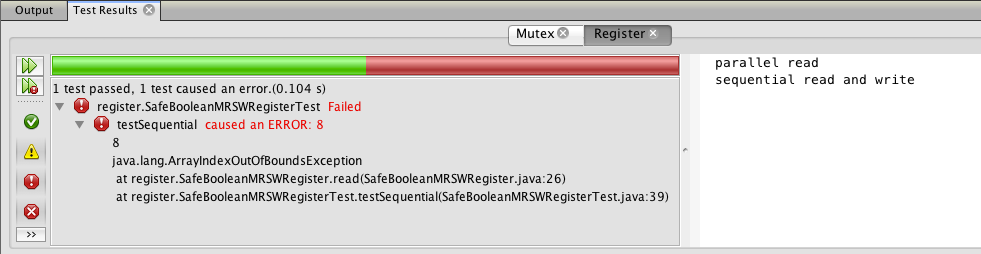
\includegraphics[width=13cm]{SafeBooleanMRSW00.png}
  \caption{First type of failure}
  \label{fig:SafeBooleanMRSW00}
\end{figure}
\par
\begin{figure}[h]
  \centering
  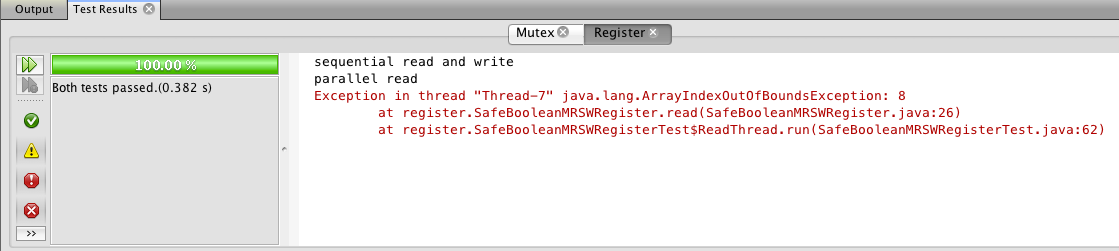
\includegraphics[width=13cm]{SafeBooleanMRSW01.png}
  \caption{Second type of failure}
  \label{fig:SafeBooleanMRSW01}
\end{figure}
\par
So, the way to fix this problem was to make sure that in each test case
the threads ids are reset calling the static method $ThreadID.reset()$. With
this hack, the tests passed (See figure \ref{fig:SafeBooleanMRSW02}).
\par
\begin{figure}[h]
  \centering
  \includegraphics[width=13cm]{SafeBooleanMRSW02.png}
  \caption{Output after fix}
  \label{fig:SafeBooleanMRSW02}
\end{figure}
\par
\begin{figure}[h]
  \centering
  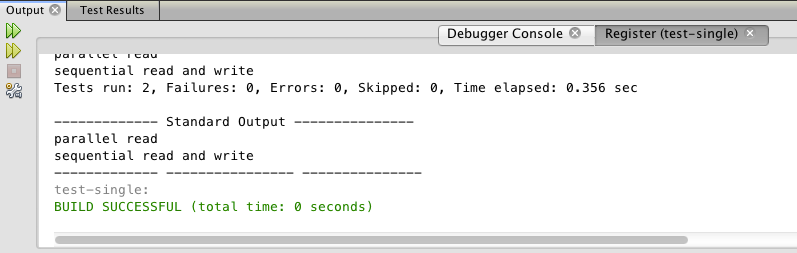
\includegraphics[width=13cm]{SafeBooleanMRSW03.png}
  \caption{Output after fix of threadIds}
  \label{fig:SafeBooleanMRSW03}
\end{figure}
\par
% ------------------------------------------------------------------------------------ %
\subsection{Interpretation}
\par
In this experiment we saw a way of implementing Safe Multi-Reader Single-Writer
registers. These registers were able of storing boolean values.
\par
Unfortunately, none of the test cases excersice the case where we have
concurrent writes and reads. Hence, this experiment only excersiced one of the
two rules of a safe register.
% ------------------------------------------------------------------------------------ %

\section{\textbf{Atomic MRSW Register}}
% -------------------------------------------------------------------------------- %
\subsection{Particular Case}
\par
The characteristics of this type of register are:
\begin{itemize}
\item It should never happen that $R^{i} \rightarrow W^{i}$
\item It should never happen that for any ${j}$, ${W^{i} \rightarrow W^{j} \rightarrow R^{j}}$
\item If ${R^{i} \rightarrow R^{j}}$ then ${i \leq j}$
\end{itemize}
The book proposes to do this by using multiple SRSW registers.
% -------------------------------------------------------------------------------- %
\subsection{Solution}
The algorithm then requires a 2 dimensional table. When a writer decides to
update the register, it has to update the values in cells $A[i][i]$, where $i$
is the thread id. Apart from writing the value, it has to also update the cell
with a timestamp. 
\par
In the other hand, when a reader wants to read from the register, it checks the
timestamp of the cell $A[i][i]$. After that, it has to check other cells in the
same column (ie, cells $A[x][i]$) to see if there has been an update in between.
That is done by comparing the timestamps. If there is a newer timestamp, the
reader has then to update all cells in its row (ie $A[i][x]$). This is the way
to indicate subsequent readers which version of the value has the previous
reader retrieved.
\par
It is easy to see that the first property is satisfied because there is no way
to read a future value. In order to read a value, this value has to be written
before.
\par
The second property is also satisfied because when a reader reads the value, it
reads the one with the most recent timestamp by scaning the timestamps in its
corresponding column. This reader also helps subsequent readers by updating all
cells in its row. Forcing property 3 to be satisfied as well.
\par
% -------------------------------------------------------------------------------- %
\subsection{Experiment Description}
\par 
The two test cases presented demonstrates the same as previous examples so we
will not describe the experiment further. 
\par
These are the details of the system we used to run the experiments:
\begin{itemize}
\item Processor: Intel Core i5 @2.5 GHz. 2 Cores.
\item L2 Cache per Core: 256 KB
\item L3 Cache: 3 MB
\item System Memory: 16 GB
\end{itemize}
% -------------------------------------------------------------------------------- %
\subsection{Sample Results}
As in previous examples, we identified that the test fails from time to time.
Figure \ref{fig:AtomicMRSW00} shows the output when the failure is seen.
\par
\par
\begin{figure}[h]
  \centering
  \includegraphics[width=13cm]{AtomicMRSW00.png}
  \caption{First type of failure}
  \label{fig:AtomicMRSW00}
\end{figure}
\par
Again, the fix for these failures was to reset the thread ids.
\par
\begin{figure}[h]
  \centering
  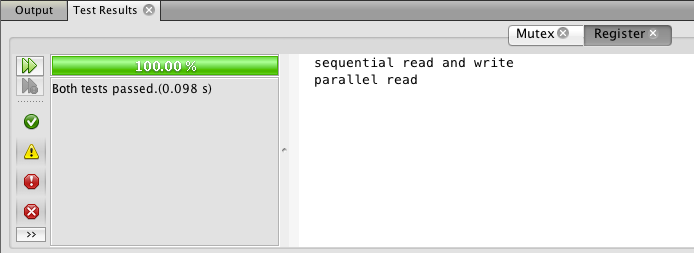
\includegraphics[width=13cm]{AtomicMRSW01.png}
  \caption{Output after fix}
  \label{fig:AtomicMRSW01}
\end{figure}
\par
\begin{figure}[h]
  \centering
  \includegraphics[width=13cm]{AtomicMRSW02.png}
  \caption{Output after fix of threadIds}
  \label{fig:AtomicMRSW03}
\end{figure}
\par
% -------------------------------------------------------------------------------- %
\subsection{Interpretation}
\par
In this experiment we observed a way of implementing MRSW registers. We saw
that, at least in the processor we used, the algorithm seems to work correctly.
\par
It would have been great, though, to also have test cases that demonstrate that this
particular register satisfies property 3 which is the one that makes it
different from the Safe version.
% -------------------------------------------------------------------------------- %

\section{\textbf{Wait-Free Snapshots}}
% ---------------------------------------------------------------------------- %
\subsection{Particular Case}
\par
In this experiment we are dealing with the problem of creating an algorithm to
create a Snapshot of a set of Register in such a way that the algorithm
guarantees a Wait-Free operation.
\par
% ---------------------------------------------------------------------------- %
\subsection{Solution}
\par
The purpose of a Wait-Free snapshot is to overcome the problems of the Simple
snapshot presented before. Let us remember that such snapshot executes successive
collect() operations. Once it achieves a \textit{clean double collect}, it
returns the snapshot. Otherwise, it uses the following idea:
\par
When a double collect fails, it is because a update interfered. That means that
the updater could take a snapshot right before its update and other threads
could use it as their snapshot too. 
\par
Since this algorithm is a bit more complex, let us explain in more detail how
the implementation works.
\par
\hfill
\begin{lstlisting}[style=numbers]
  public WFSnapshot(int capacity, T init) {
    a_table = (StampedSnap<T>[]) new StampedSnap[capacity];
    for (int i = 0; i < a_table.length; i++) {
      a_table[i] = new StampedSnap<T>(init);
    }   
  }
\end{lstlisting}
\hfill
\par
Firstly, the algorithm uses an array to store the information.
The size of the array is, in this case, $n$, where $n$ is the number of
threads. The way in which this array is constructed is as an array of
\textit{StampedSnap}s. A StampedSnap is internally an array whose elements are
of type \textit{T}. A StampedSnap is a subclass of StampedValue which has 3
fields:
\par
\begin{itemize}
\item \textit{stamp}, which is a counter
\item \textit{owner}, which contains the thread id
\item \textit{value}, the actual value in the register
\end{itemize}
\par
Now let us look at an auxiliar operation which is \textit{collect()}. This
operation returns a copy of the array. Observe that the method creates a new
array of StampedSnap values and then iterates the existing array to copy each element.
\par
\hfill
\begin{lstlisting}[style=numbers]
  private StampedSnap<T>[] collect() {
    StampedSnap<T>[] copy = (StampedSnap<T>[]) new StampedSnap[a_table.length];
    for (int j = 0; j < a_table.length; j++)
      copy[j] = a_table[j];
    return copy;
  }
\end{lstlisting}
\hfill
\par
The next method to understand is \textit{scan()}. The method first creates a
backup or an old copy of the array. Then it takes a second collect. It then
compares both copies. If both copies are equal, then it means that we have a
double clean collect. And the result of the scan operation is any of the copies
just as in the Sequential Snapshot case.
\par
On the other hand, if the copies are different, then there are two cases. For
this, we have a counter that indicates how many times, the copies have been
compared and found different. If it is the first time, then we take another
collect. If in the second collect, the copies are equal, then we fall in the
case described in the previous paragraph. If the copies are different again,
then it means that we can take the old copy as a result of the scan. 
\par
The justification of this is that if a thread A sees a thread B move twice while
it is performing repeated collects, then B executed a complete \textit{update()}
call within the interval of A's scan, and so it is correct for A to use B's
snapshot.
\par
\hfill
\begin{lstlisting}[style=numbers]
  public T[] scan() {
    StampedSnap<T>[] oldCopy;
    StampedSnap<T>[] newCopy;
    boolean[] moved = new boolean[a_table.length];
    oldCopy = collect();
    collect: while (true) {
      newCopy = collect();
      for (int j = 0; j < a_table.length; j++) {
        // did any thread move?
        if (oldCopy[j].stamp != newCopy[j].stamp) {
          if (moved[j]) {       // second move
            return oldCopy[j].snap;
          } else {
            moved[j] = true;
            oldCopy = newCopy;
            continue collect;
          }   
        }   
      }   
      // clean collect
      T[] result = (T[]) new Object[a_table.length];
      for (int j = 0; j < a_table.length; j++)
        result[j] = newCopy[j].value;
      return result;
    }   
  }
\end{lstlisting}
\hfill
\par
Finally, we have the \textit{update()} operation which simply updates the
register with the new stamp.
\par
\hfill
\begin{lstlisting}[style=numbers]
  public void update(T value) {
    int me = ThreadID.get();
    T[] snap = this.scan();
    StampedSnap<T> oldValue = a_table[me];
    StampedSnap<T> newValue =
      new StampedSnap<T>(oldValue.stamp+1, value, snap);
    a_table[me] = newValue;
  }
\end{lstlisting}
\hfill
% ---------------------------------------------------------------------------- %
\subsection{Experiment Description}
\par
In this experiment, the test looks a bit different. Let us explain how. In this
case we have two experiments:
\par
\begin{enumerate}
\item testSequential. We spawn a new thread that updates the register with a
value of \textit{FIRST} and right after that, it scans the value of the
register. The expected result is that this read retrieves the value of
\textit{FIRST}
\item testParallel. We spawn \textit{THREADS} number of threads (in our case it
is $2$). Each of them will first update its register with a value of
\textit{FIRST} and then with a value of \textit{SECOND}. Each thread then
updates a position in a matrix of size \textit{THREADS}$x$\textit{THREADS} with
the result of doing a $scan()$ operation. At the end we compare consecutive rows
in the matrix. The comparison is done entry by entry and we should see that for
some entries the first entry is greater and for some others it is smaller than
the second. What we must see is that all entries are equal and we allow the
first to sometimes be either greater or smaller than the second one.
\end{enumerate}
% ---------------------------------------------------------------------------- %
\subsection{Sample Results}
\par
For this test, we saw that in every try, both test cases passed. Here is the
output:
\par
\begin{verbatim}
[oraadm@gdlaa008 Register]$ junit register.WFSnapshotTest
.sequential
.parallel

Time: 0.003

OK (2 tests)
\end{verbatim}
\par
% ---------------------------------------------------------------------------- %
\subsection{Interpretation}
% ---------------------------------------------------------------------------- %
In this experiment we were able to observe how a Wait-Free Snapshot can be
constructed based on the idea of \textit{clean double collects} and on the idea
of using the updater's collect when the clean double collect method fails.

% --------------------------- %
% Foundations End
% --------------------------- %

% --------------------------- %
% Spin Locks Start
% --------------------------- %
\chapter{Spin Locks and Contention}
../../zava/Multiprocessor//SpinLocks.tex
../../zava/Multiprocessor//TASLockTest.tex
\section{\textbf{Hierarchical Backoff Lock}}
\subsection{Particular Case}
\par
The specific case we are trying to solve here is that of mutual exclusion with long waiting times on architectures that make use of hierarchical caching. Let us describe more deeply the characteristics of this scenario.
\par
Firstly, it has already been discussed the difference between \textit{spinning} and \textit{backing-off}. The first case consists on doing an active wait in the case where a $lock()$ operation is not successful. On the other hand, a $backoff$ means that the thread
who failed to acquire the lock refraing from retrying for some duration giving competing threads a chance to finish. As mentioned in the book, the idea is to avoid bus traffic caused by threads asking over and over again for the state of the lock.
\par
The term \textit{Hierarchical} comes from the fact that modern cache-coherent architectures organize processors in clusters. These clusters are organized in such a way that intra-cluster communication is faster than inter-cluster communication. So, the idea in this experiment is to find a lock implementation that takes advantage of these access times differences.
\par
\subsection{Solution}
\par
One of the solutions proposed in the book consists on adapting the \textit{test-and-test-and-set} lock that was described in a previous chapter to exploit the characteristics of the cluster. The idea behind this implementation is that backoff times of local threads should be shorter than backoff times of remote threads. 
\par
\subsection{Experiment Description}
\par
To demonstrate that this implementation works, the test that was provided does the following:
\begin{enumerate}
\item Initiate a shared counter with a value of $0$
\item Start $32$ threads
\item Each thread has to increment the counter by one $32$ times
\item At the end, the counter must hold a value of $32*32$
\end{enumerate}
\par
These are the details of the system we used to run the experiments:
\begin{itemize}
\item Processor: Intel Core i5 @2.5 GHz. 2 Cores.
\item L2 Cache per Core: 256 KB
\item L3 Cache: 3 MB
\item System Memory: 16 GB
\end{itemize}
\subsection{Sample Results}
\par
For this test, we saw that in every try, it always passed.
\par
\begin{figure}[h]
  \centering
  \includegraphics[width=5cm]{HBO00.png}
  \caption{Successful execution of the tests for Hierarchichal Back-off test}
  \label{fig:HBO00}
\end{figure}
\par
\begin{figure}[h]
  \centering
  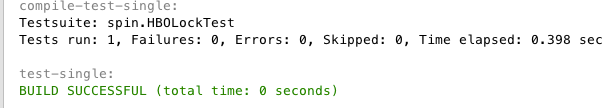
\includegraphics[width=13cm]{HBO01.png}
  \caption{Successful execution of the tests  for Hierarchichal Back-off test}
  \label{fig:HBO01}
\end{figure}
\par
\subsection{Interpretation}
It was shown that the algorithm seems to work and allows synchronization of multiple threads trying to access a shared resource.
\par
One problem however, has to do with the fact that this locking protocol is not fair in the sense that local threads have more chances of acquiring the lock in the next attempt. 
\par
Another thing that we ought to note is that threads spin in the same memory address which causes invalidation of remote cached copies of this value. This problem will be solved yet with another protocol.

\section{\textbf{CLH Queue Lock}}
%%%%%%%%%%%%%%%%%%%%%%%%%%%%%%%%%%
\subsection{Particular Case}
\par
Using queue locks solve two problems that appear in simpler locking protocols.
Firstly, by using a queue, cache-coherence traffic is reduced because each
thread spin on a different memory location; and secondly, by using a queue,
threads can know whether their turn has come by inspecting the status of their
predecesor in the queue.
\par
The particular case that we want to study in this experiment is \textit{How can
we implemente a space efficient Queue Lock?}
\par
%%%%%%%%%%%%%%%%%%%%%%%%%%%%%%%%%%
\subsection{Solution}
\par
One solution for this problem is given by the CLHLock protocol. The algorithm
that implement this protocol need two fields local to the thread: A pointer to
the current node and a pointer to the previous node. The queue is constructed by
having the pointer \textit{previous} pointing to the previous node's
\textit{current} field. This field contains a boolean value which is false when
the thread releases the lock. When this is the case, the next thread is allowed
to acquire the lock. 
\par
%%%%%%%%%%%%%%%%%%%%%%%%%%%%%%%%%%
\subsection{Experiment Description}
\par
To demonstrate that this implementation works, the test that was provided does
the following:
\begin{enumerate}
\item Initiate a shared counter with a value of $0$
\item Start $8$ threads
\item Each thread has to increment the counter by one $1024$ times
\item At the end, the counter must hold a value of $8*1024$
\end{enumerate}
\par
%%%%%%%%%%%%%%%%%%%%%%%%%%%%%%%%%%
\subsection{Sample Results}
\par
In this case, we found that in our 24-cores machine, the test hung. To make it
work, we had to make the \textit{locked} variable in the 
\par
\hfill
\begin{verbatim}
[oraadm@gdlaa008 Spin]$ junit spin.CLHLockTest 
[8] Leaving critical zone
[9] Entering critical zone
[9] Leaving critical zone
[8] Entering critical zone
[8] Leaving critical zone
[9] Entering critical zone
[9] Leaving critical zone
[8] Entering critical zone
[9] Entering critical zone
...
[9] Leaving critical zone
[8] Entering critical zone
[9] Entering critical zone
[8] Leaving critical zone
[8] Entering critical zone
[8] Leaving critical zone

Time: 0.755

OK (1 test)
\end{verbatim}
\hfill
\par
%%%%%%%%%%%%%%%%%%%%%%%%%%%%%%%%%%
\subsection{Interpretation}
It was shown that the algorithm seems to work and allows synchronization of
Multiple threads trying to access a shared variable.
\par
One important thing about this algorith is that threads spin checking for
different memory addresses which avoids invalidation of cached copies. Another
important advantage is that it requieres a limited number of memory and also
provides first-in-first-out fairness. 
\par
The case were this algorithm is not good is when, in a NUMA architecture, the
\textit{previous} pointer points to a remote location. In that case, the
performance of the algorithm degradates.

% --------------------------- %
% Spin Locks End
% --------------------------- %

% --------------------------- %
% Monitors Start
% --------------------------- %
\chapter{Monitors and Blocking Synchronization}
../../zava/Multiprocessor//CountDownLatch.tex
% --------------------------- %
% Monitors End
% --------------------------- %

% --------------------------- %
% Linked Lists Start
% --------------------------- %
\chapter{Linked Lists: The Role of Locking}
\section{\textbf{LockFreeQueueTest}}

\subsection{Particular Case (problem)}
This is a particular case of the mutual exclusion problem, where the
shared resource is a queue.

\subsection{Solution}
In order to guarantee the correctness of
the multi-threaded access to the queue, it implements a lock free
scheme on its \C{enq} and \C{deq} methods by putting waits
before modifying the state of the queue. It does it incorrectly
though, as we will see later. \\

\begin{lstlisting}[style=numbers]
class LockFreeQueue {
  public int head = 0;   // next item to dequeue
  public int tail = 0;   // next empty slot
  Object[] items; // queue contents
  public LockFreeQueue(int capacity) {
    head = 0; tail = 0;
    items = new Object[capacity];
  }

 public void enq(Object x) {
     // spin while full
     while (tail - head == items.length) {}; // spin
     items[tail % items.length] = x;
     tail++;
  }

  public Object deq() {
      // spin while empty
      while (tail == head) {}; // spin
      Object x = items[head % items.length];
      head++;
      return x;
  }
}
\end{lstlisting}
\hfill

\subsection{Experiment Description}
The test program LockFreeQueueTest includes the following individual
test cases; the parallel degree is two threads for each operation
(queue or dequeue), with a TEST\_SIZE of 512 (number of items to
enqueue and dequeue) which is spread evenly among the two threads on
each group:

\begin{itemize}
  \item \C{testSequential}: calls \C{enq} method as many times as
    TEST\_SIZE, and later calls \C{deq} method the same number of
    times checking that the FIFO order is preserved. 
  \item \C{testParallelEnq}: enqueues in parallel (two threads) but dequeues
    sequentially.
  \item \C{testParallelDeq}: enqueues sequentially but dequeues in
    parallel (two threads)
  \item \C{testParallelBoth}: enqueues and dequeues in parallel (with
    a total of four threads, two for each operation).
\end{itemize}

\subsection{Observations and Interpretations}
The bottom line of this exercise is most likely, to show several types
of problems that can occur if we do not use mutual exclusion; the
queue implementation fails implementing it, making the test vulnerable
to several cases of race conditions. Below we explain some of them.

\subsubsection{Non atomic dequeue: referencing invalid registers}

The symptom for this problem is a NullPointerException: \\

\begin{verbatim}
There was 1 error:
1) testParallelEnq(mutex.LockFreeQueueTest)java.lang.NullPointerException
	at mutex.LockFreeQueueTest.testParallelEnq(LockFreeQueueTest.java:69)
	at sun.reflect.NativeMethodAccessorImpl.invoke0(Native Method)
	at sun.reflect.NativeMethodAccessorImpl.invoke(NativeMethodAccessorImpl.java:62)
	at sun.reflect.DelegatingMethodAccessorImpl.invoke(DelegatingMethodAccessorImpl.java:43)
\end{verbatim}
\hfill

where the offending line is a cast to an Integer from the value
returned by the \C{deq} method; this implies that such function is
returning \C{null}. A possible scenario to produce this outcome is as
follows. Prefixes of T1 or T2 indicate the thread running the action,
and they refer to the line numbers of the code of method \C{deq}
posted above.

\begin{itemize}
\item Assume that queue holds a single element which lives in \C{items}
  array at position 0; the array has \C{null} on position 1 (per
  initialization).
\item T1: Executes method up to line 20. 
\item T2: Executes method up to line 19. 
\item T1: Executes line 21, getting \C{items[0]}. 
\item T2: Executes line 20, but as \C{head} was changed already, it
  gets \C{items[1]}.  
\item T1: Executes line 22 returning \C{items[0]}
\item T2: Executes line 22 returning \C{items[1]}, which was \C{null}.
\end{itemize}
\hfill

The problem with above interlacing derives from the fact that the
\C{deq} method is not an atomic operation, hence it allowed both threads to
enter into the critical section and compete for updating the shared
variables. 

\subsubsection{Non atomic dequeue: returning duplicate values}

The symptom for this problem is a duplicate pop warning: \\

\begin{verbatim}
.parallel both
.sequential push and pop
.parallel enq
E.parallel deq
Exception in thread "Thread-7" junit.framework.AssertionFailedError: 
DeqThread: duplicate pop
	at junit.framework.Assert.fail(Assert.java:47)
	at mutex.LockFreeQueueTest$DeqThread.run(LockFreeQueueTest.java:132)
\end{verbatim}
\hfill

where the offending line is an assertion that validates that nobody
else has pop such value from the queue; as the threads which populate
do have non overlapping ranges of values, the pop operations (\C{deq})
shall never return a duplicate one. But duplication is possible
indeed, if we have a sequence like the one below between the two threads:

\begin{itemize}
\item Assume that queue holds a single element which lives in \C{items}
  array at position 0.
\item T1: Executes method up to line 19. 
\item T2: Executes method up to line 19. 
\item T1: Executes line 20, getting \C{items[0]}.
\item T2: Executes line 20, getting as well \C{items[0]}.
\item T1: Executes line 21, setting \C{head} to 1.
\item T2: Executes line 21, setting \C{head} to 2.
\item T1: Executes line 22 returning \C{items[0]}.
\item T2: Executes line 22 returning \C{items[0]}.
\end{itemize}
\hfill

Not only we left the queue in an inconsistent state (head has
incorrect value), but we also returned the same element twice,
triggering then the violation on the test. The underlying problem is
the same as previous case: lack of atomicity of the \C{deq} method.

\subsubsection{Non atomic auto-increment: loosing values}

The symptom for this problem is a never ending program, hanging on the
test \C{testParallelBoth}. When produced several thread dumps of the
Java program, we can see two hanging threads: \\

\begin{verbatim}
"Thread-7" #16 prio=5 os_prio=0 tid=0x00007f3140102000 nid=0x3f51
           runnable [0x00007f31226e9000]
   java.lang.Thread.State: RUNNABLE
	at mutex.LockFreeQueue.deq(LockFreeQueue.java:33)
	at mutex.LockFreeQueueTest$DeqThread.run(LockFreeQueueTest.java:141)

"main" #1 prio=5 os_prio=0 tid=0x00007f3140009800 nid=0x3f3c in Object.wait() 
          [0x00007f3148382000]
   java.lang.Thread.State: WAITING (on object monitor)
	at java.lang.Object.wait(Native Method)
	- waiting on <0x00000000d6effea8> (a mutex.LockFreeQueueTest$DeqThread)
	at java.lang.Thread.join(Thread.java:1245)
	- locked <0x00000000d6effea8> (a mutex.LockFreeQueueTest$DeqThread)
	at java.lang.Thread.join(Thread.java:1319)
	at mutex.LockFreeQueueTest.testParallelBoth(LockFreeQueueTest.java:123)
	at sun.reflect.NativeMethodAccessorImpl.invoke0(Native Method)
	at sun.reflect.NativeMethodAccessorImpl.invoke(NativeMethodAccessorImpl.java:62)
	at sun.reflect.DelegatingMethodAccessorImpl.invoke(DelegatingMethodAccessorImpl.java:43)
	at java.lang.reflect.Method.invoke(Method.java:497)
	at junit.framework.TestCase.runTest(TestCase.java:164)
	at junit.framework.TestCase.runBare(TestCase.java:130)
\end{verbatim}
\hfill

The main thread is waiting for a dequeue thread to finish; but that
one is on an infinite loop at line 19 of \C{deq} method (line numbers
per our listing in this document, not in the file). This means that we
have lost some of the inserted elements in queue, and that one of the
dequeue threads will never finish; as they expect each to pop a fixed
amount of elements per the test. \\

But the amount of times we request a dequeue operation, among all
threads, is the same as the number of elements we queued; how come we
end up loosing some of those? One possible explanation is again, the
lack of atomicity but this time of the \C{enq} method; to be more
specific, the lack of atomicity of its auto-increment operation 
\C{tail++} (line 14). Let us remember that the auto-increment
operator in Java is nothing but syntactic sugar for the following
sequence of operations (when applied to \C{tail} variable): \\

\begin{lstlisting}[style=nonumbers]
  tmp = tail;
  tmp = tmp + 1;
  tail = tmp;
\end{lstlisting} 
\hfill

If two threads execute the lower level operations above, we can see
how they can end up loosing increments in the shared variable
\C{tail}; the following sequence is on example of such scenario:

\begin{itemize}
\item T1: executes \C{tmp = tail}.
\item T2: executes \C{tmp = tail}.
\item T1: executes \C{tmp = tmp + 1}.
\item T2: executes \C{tmp = tmp + 1}.
\item T1: executes \C{tail = tmp}.
\item T2: executes \C{tail = tmp}.
\end{itemize}
\hfill

We can appreciate that in the above interlacing, the final value of
the shared variable is $\C{tail} + 1$; instead of the expected value
of $\C{tail} + 2$. It would be enough to loose a single value this
way, in order to make the enqueue threads think that they inserted the
total of 512, while they really inserted 511; as each dequeue thread
will try to pop 256 each, only one of them will be able to finish
while the other will get blocked after having removed 255
entries. That is most likely the explanation for the hung threads we
pasted above \footnote{Note that it does not matter that the array
  \C{items} has populated all the correct entries, because the flow is
  controlled by the counters \C{tail} and \C{head}.}; the solution is
again to really implement mutual 
exclusion around the methods \C{deq} / \C{enq}; in such a way that
they become atomic operations.

\subsection{Proposed changes to fix the problems}

All the three scenarios described before can be eliminated, if we make
the methods \C{enq} and \C{deq} atomic; this can be easily achieved in
Java by making them \C{synchronized}. However, by doing that, we will
loose parallelism among the two groups of threads (those calling
\C{enq} and those calling \C{deq}); this is because the
\C{synchronized} keyword uses as lock the whole object, so at any
moment in time, only one synchronized method can actually run within any object. In
order to overcome this limitation, we can use synchronized blocks
against two different lock objects (one for each operation). \\

Even with the changes above, we can still have issues; what if the
very first thread running is one calling \C{deq} method? It will find
the queue empty and loop forever. In order to prevent that, we should
remove the waiting operation out of the queue methods, and put them in
the test code itself. This is because, on the cited scenario that we
try to dequeue with an empty queue, we would expect to simply try
again (giving the chance to parallel enqueue threads to produce something for
us to pop). The final code which incorporates these fixes is listed
below: \\

\newpage
\begin{lstlisting}[style=numbers]
class LockFreeQueue {
  private static Object enqLock = new Object();
  private static Object deqLock = new Object();
    
  public int head = 0;   // next item to dequeue
  public int tail = 0;   // next empty slot
  Object[] items; // queue contents
  public LockFreeQueue(int capacity) {
    head = 0; tail = 0;
    items = new Object[capacity];
  }

 public  boolean enq(Object x) {
     synchronized(enqLock)
         {
             if (tail - head == items.length) {
                 return false;
             }
             items[tail % items.length] = x;
             tail++;
             return true;
         }
  }

  public Object deq() {
      synchronized(deqLock)
          {
              if (tail == head) {
                 return null;
              }
              Object x = items[head % items.length];
              head++;
              return x;
          }
  }
}

\end{lstlisting}
\hfill
\newpage

The test code was also modified, to make the enqueue and dequeue
threads to iterate until they have successfully called their
respective methods 256 times (total size of queue divided by number of
threads). A successful call is one that does not return \C{false} nor
\C{null}. The modified code was executed ten thousand times and it did
not produce any of the original problems we explained. Though not a
formal proof of its correctness, it is a good indication of the same
(the original program produced one of the cited problems quite often,
usually within 10 executions).



\section{\textbf{LazyListTest}}

\subsection{Particular Case (problem)}
The problem is that of gradually improving what coarse grain locking
offers for concurrent data structures like sets (implemented with
linked lists).

\subsection{Solution}
The \C{LazyList} solution is a refinement of the \C{OptimisticList}
solution which does not lock while searching, but locks one it finds
the interesting nodes (and then confirms that the locked nodes are
correct). As one drawback of \C{OptimisticList} is that the most
common method \C{contains} method locks, the next logical improvement
is to make this method wait-free while keeping the \C{add} and
\C{remove} methods locking (but reducing their transversings of the
list from two to just one). \\

The refinement mentioned above is precisely that of \C{LazyList},
which adds a new bit to each node to indicate whether they still
belong to the set or not (this prevents transvering the list to detect
if the node is reachable, as the new bit introduces such invariant: if
a transversing thread does not find a node or it is marked in this
bit, then the corresponding item does not belong to the set. This
behavior implies that \C{contains} method does a single wait-free
transversal of the list. \\

For adding an element to the list, \C{add} method traverses the list,
locks the target's predecessor and successor nodes, and inserts the
new node in between. The \C{remove}   
method is lazy (hence the name of the solution), as it splits its task in
two parts: first marks the node in the new bit, logically removing it;
and second, update its predecessor's next field, physically removing
it. \\

The three methods ignore the locks while transversing the list,
possibly passing over both logically and physically deleted nodes. The
\C{add} and \C{remove} methods still lock \C{pred} and \C{curr} nodes
as with \C{OptimisticList} solution, but the validation reduces to
check that \C{curr} node has not been marked; as well as validating
the same for \C{pred} node, and that it still points to \C{curr}
(validating a couple of nodes is much better than transversing whole
list though). Finally, the introduction of logical removals implies a
new contract for detecting that an item still belongs to set: it does
so, if still referred by an unmarked reachable node. \\

The most relevant methods, \C{remove} and \C{contains}, are listed
below: \\

\begin{lstlisting}[style=numbers]
  public boolean remove(T item) {
    int key = item.hashCode();
    while (true) {
      Node pred = this.head;
      Node curr = head.next;
      while (curr.key < key) {
        pred = curr; curr = curr.next;
      }
      pred.lock();
      try {
        curr.lock();
        try {
          if (validate(pred, curr)) {
            if (curr.key != key) {    // present
              return false;
            } else {                  // absent
              curr.marked = true;     // logically remove
              pred.next = curr.next;  // physically remove
              return true;
            }
          }
        } finally {                   // always unlock curr
          curr.unlock();
        }
      } finally {                     // always unlock pred
        pred.unlock();
      }
    }
  }

  public boolean contains(T item) {
    int key = item.hashCode();
    Node curr = this.head;
    while (curr.key < key)
      curr = curr.next;
    return curr.key == key && !curr.marked;
  }
\end{lstlisting}
\hfill

\subsection{Experiment Description}
The test is pretty much the same described for \C{LockFreeQueueTest},
with a few differences.

\begin{itemize}
\item The data structure here is a set, rather than a queue.
\item The exception that it uses 8 threads instead of two for each
  operation (\C{add} / \C{remove}).
\item The threads that remove elements do not care only in
  successfully removing certain number of times (like with the queue);
  here they expect to remove a particular subset of the values.
\end{itemize}
  

\subsection{Observations and Interpretations}

The test works as expected on a two cores machine, sample output below:

\begin{verbatim}
.parallel deq
.parallel both
.sequential push and pop
.parallel enq

Time: 0.03

OK (4 tests)
\end{verbatim}
\hfill

Interestingly, on a 24 cores machine, sometimes the test case
\C{testParallelBoth} fails with exceptions like the one below: \\

\begin{verbatim}
junit.framework.AssertionFailedError: RemoveThread: duplicate remove
at junit.framework.Assert.fail(Assert.java:57)
at junit.framework.TestCase.fail(TestCase.java:227)
at lists.LazyListTest$RemoveThread.run(LazyListTest.java:142)
\end{verbatim}
\hfill

While debugging the error above, we found that the message of
``duplicate remove'' is a bit misleading; is not really that someone
else tried to delete that value (as each \C{RemoveThread} cares about
a unique set of values). The real problem is that the removing threads
just try once to remove each value, and fail if they did not find any
of them. Since both the adder and remover threads are started
concurrently, there is no guarantee that the adders will come first
than the removers; so it could be that the removers try to pull out
something that has not been inserted yet (leaving to the exception
shown above). \\

Since the \C{LazyList} solution does not include an error-and-retry
approach (as with our second rewrite of the \C{LockFreeQueue}, which
used Java condition's await methods), the only way to fix this would
be to rewrite the test program itself. Each remover thread will need
to indefinitely try to remove all its items until completion, rather
than expecting that all of them are available by the time they are to
be removed. We tried that approach and made the proper adjustments
to the test program, after which the problem got solved as expected.

%\section{\textbf{Coarse List}}
% ---------------------------------------------------------------------------- %
\subsection{Particular Case}
\par
In this experiment we are dealing with the problem of creating an algorithm to
create a Snapshot of a set of Register in such a way that the algorithm
garantees a Wait-Free operation.
\par
% ---------------------------------------------------------------------------- %
\subsection{Solution}
\par
The purpose of a Wait-Free snapshot is to overcome the problems of the Simple snapshot presented before. Let us remember that such snapshot executes sucesive collect() operations. Once it achieves a \textit{clean double collect}, it returns the snapshot. Otherwise, it keeps trying. 
\par
One of the ideas behind the Wait-Free Snapshot is that when a double collect fails, it is because a update interfered. That means that the updater could take a snapshot right before its update and other threads could use it as their snapshot too. 
\par
% ---------------------------------------------------------------------------- %
\subsection{Experiment Description}
\par

\par
These are the details of the system we used to run the experiments:
\begin{itemize}
\item Processor: Intel Core i5 @2.5 GHz. 2 Cores.
\item L2 Cache per Core: 256 KB
\item L3 Cache: 3 MB
\item System Memory: 16 GB
\end{itemize}
% ---------------------------------------------------------------------------- %
\subsection{Sample Results}
\par
For this test, we saw that in every try, both test cases passed.
\par
\begin{figure}[h]
  \centering
  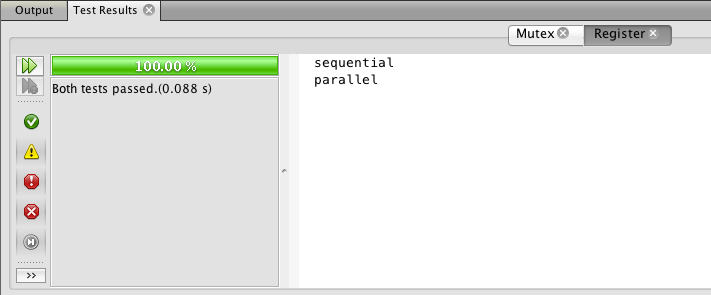
\includegraphics[width=13cm]{WFS00.png}
  \caption{Successful execution of the tests for Wait-Free Snapshot}
  \label{fig:WFS00}
\end{figure}
\par
\begin{figure}[h]
  \centering
  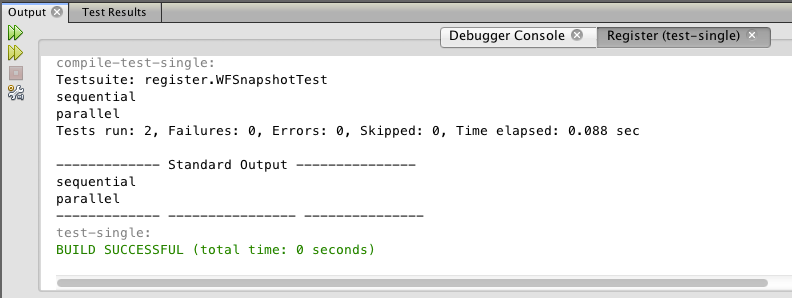
\includegraphics[width=13cm]{WFS01.png}
  \caption{Successful execution of the tests for Wait-Free Snapshot}
  \label{fig:WFS01}
\end{figure}
\par
% ---------------------------------------------------------------------------- %
\subsection{Interpretation}
% ---------------------------------------------------------------------------- %
In this experiment we were able to observe how a Wait-Free Snapshot can be
constructed. 

%\section{\textbf{Lock-Free List}}
% ---------------------------------------------------------------------------- %
\subsection{Particular Case}
\par
We have seen some algorithms for implementing a concurrent list. Now it is time
to see how a Lock-Free implementation can be done.
\par
% ---------------------------------------------------------------------------- %
\subsection{Solution}
\par
\par
% ---------------------------------------------------------------------------- %
\subsection{Experiment Description}
\par
Again, we have the same four test cases that we have been dealing with:
\par
\begin{enumerate}
\item \textit{testSequential()}. The main thread inserts multiple elements to
the list, then checks if all elements are there and finally removes all elements
one by one.
\item \textit{testParallelAdd()}. The main thread spawns multiple threads that
add elements to the list concurrently. When they are done, the main thread
checks if all elements are in there and finally removes all elements.
\item \textit{testParallelRemove()}. The main thread inserts multiple elements
to the list, then checks if all elements are in there and finally it spawns
multiple threads that remove the elements from the list concurrently.
\item \textit{testParallelBoth()}. The main thread creates multiple threads.
Some of them insert elements to the list and some of them remove elements.
\end{enumerate}
\par
% ---------------------------------------------------------------------------- %
\subsection{Sample Results}
\par
Similar to the other implementations, the test cases turns out to have a
problem. Here is the output:
\par
\begin{verbatim}
[oraadm@gdlaa008 Lists]$ junit lists.LockFreeListTest
.sequential add, contains, and remove
.parallel both
Exception in thread "Thread-13" junit.framework.AssertionFailedError:
RemoveThread: duplicate remove: 109
        at junit.framework.Assert.fail(Assert.java:57)
        at junit.framework.TestCase.fail(TestCase.java:227)
        at lists.LockFreeListTest$RemoveThread.run(LockFreeListTest.java:145)
.parallel add
.parallel remove

Time: 0.022

OK (4 tests)
\end{verbatim}
\par
The fix for this is the same that has been discussed before. Here is the test
output after the fix:
\begin{verbatim}
[oraadm@gdlaa008 Lists]$ junit lists.LockFreeListTest
.sequential add, contains, and remove
.parallel both
.parallel add
.parallel remove

Time: 0.016

OK (4 tests)
\end{verbatim}
\par
% ---------------------------------------------------------------------------- %
\subsection{Interpretation}
% ---------------------------------------------------------------------------- %
We observed a way in which a list could be implemented allowing it to be lock
free. When using the same set of unit tests as before, we see that the
implementation works correctly.

% --------------------------- %
% Linked Lists End
% --------------------------- %

% --------------------------- %
% Concurrent Queues Start
% --------------------------- %
\chapter{Concurrent Queues and the ABA Problem}
../../dario/Multiprocessor//SynchronousDualQueueTest.tex
\section{\textbf{LockFreeQueueRecycleTest}}

\subsection{Particular Case (problem)}
From the generic problem of improving coarse grained lock approaches,
the particular approach followed on this exercise corresponds to the
extreme case: lock-free data structure. The particular case is for a
queue, and it has the additional bonus of recycling memory.

\subsection{Solution}
The solution is based on an 1996 ACM article from Maged M. Michel and
Michael L. Scott, who based on previous publications, suggest a new
way of implementing a lock-free queue with recycles. They implement the
queue with a single-linked list using \C{tail} and \C{head} pointers;
where \C{head} always points to a dummy or sentinel node which is the
first in the list, and \C{tail} points to either the last or second to
last node in the list. The algorithm uses ``compare and swap''
(\C{CAS}) with modification counters to avoid the ABA problem. \\

Dequeuers are allowed to free dequeued nodes by ensuring that \C{tail}
does not point to the dequeued node nor to any of its predecessors
(that is, dequeued nodes may be safely reused). To obtain consistent
values of various pointers the authors relied on sequences of reads
that re-check earlier values to ensure they have not changed (these
reads are claimed to be simpler than snapshots). 

\subsection{Experiment Description}
The test is pretty much the same described for \C{LockFreeQueueTest}
(with the exceptiont that it uses 8 threads instead of two).

\subsection{Observations and Interpretations}
The test does not exhibit any pitfall, which suggests that the theory
works just fine on the tested machine. Sample output below:

\begin{verbatim}
.parallel enq
.parallel deq
.parallel both
.sequential push and pop

Time: 0.023

OK (4 tests)
\end{verbatim}
\hfill


\newpage
\section{\textbf{BoundedQueueTest}}

\subsection{Particular Case (problem)}
The problem is to implement a bounded partial queue (that is, one
which finite capacity which allows waits inside its methods). 

\subsection{Solution}
The solution proposes to allow concurrency among enqueuers and
dequeuers, by using two different locks (one for each group of
threads). The code is small enough to be placed and explained in a bit
more detail here, so let us give it a try:

\begin{lstlisting}[style=numbers]
  public void enq(T x) {
    if (x == null) throw new NullPointerException();
    boolean mustWakeDequeuers = false;
    enqLock.lock();
    try {
      while (size.get() == capacity) {
        try {
          notFullCondition.await();
        } catch (InterruptedException e) {}
      }
      Entry e = new Entry(x);
      tail.next = e;
      tail = e;
      if (size.getAndIncrement() == 0) {
        mustWakeDequeuers = true;
      }
    } finally {
      enqLock.unlock();
    }
    if (mustWakeDequeuers) {
      deqLock.lock();
      try {
        notEmptyCondition.signalAll();
      } finally {
        deqLock.unlock();
      }
    }
  }
\end{lstlisting}
\hfill

The main points of algorithm above are as follows (the code above was
previously corrected, as it had several things inverted):

\begin{itemize}
\item It does not allow null values.
\item There is a lock dedicated to \C{enq} method, which guarantees
  mutual exclusion to the critical section for enqueuers.
\item It spins while the queue is full (the try/catch block was added
  just to allow compilation). This line was incorrectly asking whether
  queue was empty, while it needs to ask whether is still full.
\item  Once we know queue is room, we allocate the new node and update
  \C{tail} pointer.
\item We atomically get and increment the atomic counter for the size
  (this was previously a decrement, which was incorrect).
\item If the atomically retrieved previous value of size was zero, it
  means the queue was empty and there may had been waiting dequeuers;
  therefore we acquire the lock for \C{deq} method and inform all
  dequeuers that the queue has not at least an item.
\end{itemize}
\hfill

The \C{deq} method is symmetric so we do not repeat same explanation
(but worth to say that it had same inverted conditions and actions
than \C{enq} method, in the code; so we needed to apply same
corrective actions ... perhaps that was the purpose of the exercise?).

\subsection{Experiment Description}
The test is pretty much the same described for \C{LockFreeQueueTest}.
(with the exceptiont that it uses 8 threads instead of two).

\subsection{Observations and Interpretations}
The original code for the test made no sense, as conditions and
actions for \C{enq} and \C{deq} methods were inverted; we did not even
care testing such strange version that did not match at all the one
published on the book (we also needed to fix the initialization of the
\C{size} variable, which shall be zero instead of \C{capacity}). After
the corrections mentioned on the Solution section above, the test ran
normally. Sample output below: 

\begin{verbatim}
.parallel both
.sequential push and pop
.parallel enq
.parallel deq

Time: 0.028

OK (4 tests)
\end{verbatim}
\hfill

Even if the original version of this test actually ran (we did not
test it), it turns out quite counter-intuitive. The modified code worked fine
on both 2 and 24 core machines.



% --------------------------- %
% Concurrent Queues End
% --------------------------- %

% --------------------------- %
% Counting/Sorting Start
% --------------------------- %
\chapter{Counting, Sorting and Distributed Coordination}
\section{\textbf{TreeTest}}

\subsection{Particular Case (problem)}
This problem belongs to chapter 12, where the idea is to present
problems which look inherently serial but that surprisingly accept
interesting concurrent solutions (though not always easy to
explain). The particular problem this test is exercising is that of
shared 
counting, where we have \C{N} threads to increase a shared numeric
variable up to certain value; but with the goal of producing less
contention than a serial solution would generate. 

\subsection{Solution}

The java program is called \C{Tree.java}, although it corresponds to  
the \C{CombiningTree} from the book, which is a binary tree structure
where each thread is located at a leaf and at most two threads can
share a leaf. The shared counter is at the root of the tree, and the
rest of the nodes serve as intermmediate result points. When a couple
of threads collide in their attempt to increment, only one of them
will serve as the representant and go up in the tree with the mission
of propagating the combined increment (2) up to the shared counter at
the root of the tree. In its way up, it may encounter further threads
that collide again with it, making it wait or continue its journey to
the root. \\

When a thread reaches the root it adds its accumulated result to the
shared counter, and propagates down the news that the job is done to
the rest of the threads that waited along the way. This
solution to the counting problem has worse latency than lock-based
solutions (\bigO{1} vs \bigO{log(p)}, where $p$ is the number of
threads or processors; but it offers a better throughput. 

\subsection{Experiment Description}

The program consists of a single unit test \C{testGetAndIncrement},
which creates 8 threads to perform each $2^20$ increments. The program
uses an auxiliary array called \C{test} to record the individual
increments done by each thread; assertions are made to ensure that
none of the attemtps results in a duplicated value, as well as to
ensure that all threads completed their task.

\subsection{Observations and Interpretations}

The test performs without much controversy in an elapsed time between
3 and 4 seconds (laptop computer with i5 processor). Below a sample
output: 

\begin{verbatim}
.Parallel, 8 threads, 1048576 tries

Time: 3.641
\end{verbatim}

To make the test a little more interesting, we created another couple
of tests reusing sample template of existing one; difference was the
Thread class used on each case. \\

The first additional test uses a thread class based on Java provider \\
\C{java.util.concurrent.atomic.AtomicInteger}: \\

\begin{lstlisting}[style=nonumbers]
  cnt2 = new AtomicInteger();

  class MyThread2 extends Thread {
    public void run() {
      for (int j = 0; j < TRIES; j++) {
        int i = cnt2.getAndIncrement();
        if (test[i]) {
          System.out.printf("ERROR duplicate value %d\n", i);
        } else {
          test[i] = true;
        }
      }
    }        
  }
\end{lstlisting}
\hfill

while the second additional test was based on a custom class that used
synchronized \C{getAndIncrement} method:\\

\begin{lstlisting}[style=nonumbers]
  class MyThread3 extends Thread {
    public void run() {
      for (int j = 0; j < TRIES; j++) {
        int i = cnt3.getAndIncrement();
        if (test[i]) {
          System.out.printf("ERROR duplicate value %d\n", i);
        } else {
          test[i] = true;
        }
      }
    }        
  }

  class MyCounter {
    private int cnt = 0;

    public synchronized int getAndIncrement()
    {
      return cnt++;
    }
  }
\end{lstlisting}
\hfill

The expectation was that the test test based on a synchronized method
would be the slowest (\C{Parallel3} label on output), the one based on
the \C{CombineTree} would become second (\C{Parallel1} label on
output) and the fastest would be the one based on \C{AtomicInteger}
(\C{Parallel2}); as the latest is likely to take advantage of hardware
atomic instruction of 32bits. Surprisingly, the test based on
\C{CombineTree} was the worst of all, by far: \\

\begin{verbatim}
.Parallel1, 8 threads, 1048576 tries took 3878
.Parallel2, 8 threads, 1048576 tries took 162
.Parallel3, 8 threads, 1048576 tries took 723

Time: 4.827

OK (3 tests)
\end{verbatim}
\hfill

Most likely we are not comparing apples with apples, as the theory
does not match the experiment; perhaps the \C{CombineTest} class is
not meant for real usage, so this comparison is not fair. Anyway, the
test does not hang nor fails on neither the 2 cores nor the 24 machines.






% --------------------------- %
% Counting/Sorting End
% --------------------------- %

\end{document}
